\begin{figure}[t]
	\centering
	\scalebox{0.8}{\begin{tikzpicture}[
    % define styles 
    clear/.style={ 
        draw=none,
        fill=none
    },
    net/.style={
        matrix of nodes,
        nodes={ draw, circle, inner sep=3pt },
        nodes in empty cells,
        column sep=1cm,
        row sep=.1cm
    },
    >=latex
]
% define matrix mat to hold nodes
% using net as default style for cells
\matrix[net] (mat)
{
% Define layer headings
   |[clear]| \parbox{1.5cm}{\centering $\langle x_1 \geq -1$, \\ $x_1 \leq 1$, \\ $l_1 = -1$, \\ $u_1 = 1 \rangle$} 
   & |[clear]| \parbox{2cm}{\centering $\langle x_3 \geq x_1 + x_2$, \\ $x_3 \leq x_1 + x_2$, \\ $l_3 = -2$ \\ $u_3 = 2 \rangle$}
   & |[clear]| \parbox{2.2cm}{\centering $\langle x_5 \geq 0$, \\ $x_5 \leq 0.5.x_3 + 1$, \\ $l_5 = 0$, \\ $u_5 = 2 \rangle$}
   & |[clear]|  \parbox{1.5cm}{\centering $\langle x_7 \geq x_5$, \\ $x_7 \leq x_5$, \\ $l_1 = 0$, \\ $u_1 = 2 \rangle$} \\
        
$x_1$  & $x_3$  & $x_5$ & $x_7$ \\
|[clear]| & |[clear]| & |[clear]| & |[clear]| \\
|[clear]| & |[clear]| & |[clear]| & |[clear]| \\
|[clear]| & |[clear]| & |[clear]| & |[clear]| $0.2$ \\
$x_2$  & $x_4$  & $x_6$ & $x_8$ \\
|[clear]| \parbox{1.5cm}{\centering $\langle x_2 \geq -1$, \\ $x_2 \leq 1$, \\ $l_2 = -1$, \\ $u_2 = 1 \rangle$} 
& |[clear]| \parbox{2cm}{\centering $\langle x_4 \geq x_1 + x_2$, \\ $x_4 \leq x_1 + x_2$, \\ $l_4 = -2$ \\ $u_4 = 2 \rangle$}
& |[clear]| \parbox{2.2cm}{\centering $\langle x_6 \geq 0$, \\ $x_6 \leq 0.5.x_4 + 1$, \\ $l_6 = 0$, \\ $u_6 = 2 \rangle$}
& |[clear]| \parbox{1.5cm}{\centering $\langle x_8 \geq x_6$, \\ $x_8 \leq x_6$, \\ $l_1 = 0$, \\ $u_1 = 2 \rangle$} \\
};

% left most lines into input layers
\draw[<-] (mat-2-1) -- +(-1cm,0) node[pos=1, above] {$[-1,1]$};
\draw[<-] (mat-6-1) -- +(-1cm,0) node[pos=1, above] {$[-1,1]$};

\draw[->] (mat-2-1) -- (mat-2-2) node[pos=0.5, above] {$1$};
\draw[->] (mat-2-1) -- (mat-6-2) node[pos=0.25, above] {$1$};
\draw[->] (mat-6-1) -- (mat-2-2) node[pos=0.25, above] {$1$};
\draw[->] (mat-6-1) -- (mat-6-2) node[pos=0.5, above] {$1$};

\draw[->] (mat-2-2) -- (mat-2-3) node[pos=0.5, above] {$max(0,x_3)$};
\draw[->] (mat-6-2) -- (mat-6-3) node[pos=0.5, above] {$max(0,x_4)$};

\draw[->] (mat-2-3) -- (mat-2-4) node[pos=0.5, above] {$1$};
\draw[->] (mat-2-3) -- (mat-6-4) node[pos=0.25, above] {$0$};
\draw[->] (mat-6-3) -- (mat-2-4) node[pos=0.25, above] {$0$};
\draw[->] (mat-6-3) -- (mat-6-4) node[pos=0.5, above] {$1$};


%\draw[->] (mat-2-4) -- +(1cm,0) node[pos=1, above] {$[0,3]$};
%\draw[->] (mat-6-4) -- +(1cm,0) node[pos=1, above] {$[-2,2]$};



% lines from a_{i}^{1} to a_{0}^{2}
%\foreach \ai in {1,2}
%  \draw[->] (mat-\ai-2) -- (mat-6-3);
   
% right most line with Output label
%\draw[->] (mat-6-3) -- node[above] {Output} +(2cm,0);
\end{tikzpicture}
}
	\caption{Hypothetical example of neural network}
	\label{fig:motivating}
\end{figure}
Consider a neural network in figure~\ref{fig:motivating},  which has one input, one hidden, and one output layer. The hidden layer is separated into two layers 
\affine{} and \relu{}, so a total of four layers is shown in figure~\ref{fig:motivating}. 
Every layer contains two neurons. The neuron $x_8$ has a bias of $1$, and all the other neurons have a bias of $0$. 
Our goal is to verify for all input $x_1,x_2 \in [-1,1]$ the outputs satisfy $x_7 \leq x_8$. 
Our approach extends \deeppoly{}~\cite{singh2019abstract}.
\deeppoly{} maintains one upper and
one lower constraint and an upper and lower bound for each neuron.
For a neuron of the affine layer, the upper and lower constraint is 
the same, which is the weighted sum of the input neurons i.e. $x_3$'s upper and lower constraint is $x_1+x_2$.
For an activation neuron, the upper and lower expression is computed using triangle approximation~\cite{singh2019abstract}, 
which is briefly explained in Section~\ref{sec:deeppoly}. To verify the property $x_7 \leq x_8$, \deeppoly{} creates a 
new expression $x_9 = x_7 - x_8$ and computes the upper bound of $x_9$. The upper bound of $x_9$ should not be greater
than $0$. \deeppoly{} computes the upper bound of $x_9$ by back substituting the expression of $x_7$ and $x_8$ 
from the previous layer.
They continue back substituting until only input layer variables are left.
The process of back substitution is shown in equation (1). %~\ref{eq:deeppoly}.
After back substitution, the upper bound of $x_9$ is
computed as $1$, which is greater than $0$, 
hence, the \deeppoly{} fails to verify the property.

\hspace*{-1cm}
\fbox{
\noindent\begin{minipage}{.23\linewidth}
\begin{equation*}
    \begin{aligned}
        x_9 \leq  &  x_7 - x_8 &\\
        x_9 \leq  & x_5 - x_6 - 1 \\
        x_9 \leq  & 0.5x_3 + 1 - 1 &\\
        x_9 \leq  & 0.5(x_1+x_2) \\
        x_9 \leq  & 1\\
        (1)
   \end{aligned}
%\label{eq:deeppoly}
\end{equation*}
\end{minipage}}\quad
\fbox{
\begin{minipage}{.68\linewidth}
\begin{equation*}
    \begin{aligned}
      -1 \leq & x_1 \leq 1 \hspace*{-1cm}&  \hspace*{-2cm}
      -1 \leq & x_2 \leq 1 \\
         x_1 + x_2 \leq & x_3 \leq x_1 + x_2 \hspace*{-1cm}& \hspace*{-2cm}
         x_1 + x_2 \leq & x_4 \leq x_1 + x_2 \\
         0 \leq & x_5 \leq 0.5x_3+1 \hspace*{-1cm}&  \hspace*{-2cm}
         0 \leq & x_6 \leq 0.5x_4 + 1 \\
         x_5 \leq & x_7 \leq x_5 \hspace*{-1cm}&\hspace*{-2cm}
         x_6+1 \leq & x_8 \leq x_6+1 \\
         x_7 & > x_8 \text{ (negation of property)}&&\\
        & \hspace*{2cm}(2) &&
    \end{aligned}
%\label{eq:conjunction}
\end{equation*}

\end{minipage}
}  

There are two main reasons for the failure of \deeppoly{}. First, it cannot maintain the complete correlation 
between the neurons. In this example, neurons $x_3$ and $x_4$ have the same expression $x_1+x_2$, so they always
get the same value. However, in the \deeppoly{} analysis process, it may fail to get the same value. Second, it uses triangle
approximation on \relu{} neurons.
We take the conjunction of upper and lower expressions of each neuron with the negation of the property
as shown in equation (2) %~\ref{eq:conjunction},
 and use the \milp{} solver to check satisfiability, thus addressing the first issue.  
The second issue can be resolved either by splitting the bound at zero of the 
affine node or by using the exact encoding (eq~\ref{eq:reluexact}) 
instead of triangle approximation. 
But both solutions increase the problem size exponentially in terms of \relu{} neurons and this results in a huge 
blowup if we repair every neuron of the network. 

So, the main hurdle toward efficiency is to find the set of important neurons (we call these {\em marked neurons}), 
and only repair these.  For this, we crucially use the satisfying assignment obtained from the \milp{} solver.
%When \deeppoly{} fails to verify the network, we use an \milp{} solver to check the satisfiability of equation~\ref{eq:conjunction}. 
%If it returns \unsat{} it means the property is verified otherwise we get the satisfying assignment of each variable. 
For instance, a possible satisfying assignment of equation~(2)%\ref{eq:conjunction}
is in equation~\ref{eq:sat1}. We execute the neural network with the inputs $x_1=1,x_2=1$ and get the values 
on each neuron as shown in equation~\ref{eq:sat2}. 
Then we observe that the output values $x'_7=2, x'_8=3$ satisfy the property, 
so, the input $x_1=1, x_2=1$ is a spurious counterexample. 
The question is to identify the neuron whose abstraction lead to this imprecision.
%\vspace{-20mm}
\setcounter{equation}{2}
\begin{align}
  x_1=1, x_2=1, x_3=2, x_4=2, x_5=2, x_6=0, x_7=2, x_8=1 \label{eq:sat1} \\
  x'_1=1, x'_2=1, x'_3=2, x'_4=2, x'_5=2, x'_6=2, x'_7=2, x'_8=3 \label{eq:sat2}
\end{align}

%We have to remove spurious counter example by doing the refinement analysis. 
%We are using one approach to find the marked neurons guided by the spurious counter example,  and one approach to refine (repair) the marked neurons.

% We are using two approaches to find the marked neurons guided by the spurious counter example, 
% and two approaches to refine (repair) the marked neurons.
% \begin{equation}
%     \begin{aligned}
%         x_1=1, x_2=1, x_3=2, x_4=2, x_5=2, x_6=0, x_7=2, x_8=1\\
%     \end{aligned}
%         \label{eq:sat1}
% \end{equation}

% \begin{equation}
%     \begin{aligned}
%         x'_1=1, x'_2=1, x'_3=2, x'_4=2, x'_5=2, x'_6=2, x'_7=2, x'_8=3
%     \end{aligned}
% \label{eq:sat2}
% \end{equation}


%Following is the approach to find the marked neurons.
%\\
\noindent\textbf{Maxsat based approach to identify marked neurons}\\
%The satisfying assignments of equation~\ref{eq:conjunction} are in equation~\ref{eq:sat1}. We execute the satisfying assignment $x_1=1,x_2=1$ on the neural network and get values on each neuron as  shown in equation~\ref{eq:sat2}.
% We make the point on \texttt{relu} layer in eq~\ref{eq:sat1} as close as possible to the point 
% of \texttt{relu} in equation~\ref{eq:sat2} by encoding them as soft constraints (i.e.,  $\{x_5=2, x_6=2\}$) 
% while maintaining that the rest of the hard constraints are satisfied (see Equation~\ref{eq:opt1})
% e.g., input points $x_1,x_2$ and output points $x_7,x_8$ are the same etc. 
% %The soft constraints define the closeness point on the relu layer of equations~\ref{eq:sat1} and \ref{eq:sat2}. 
% Then we feed this to a maxsat solver \todo{check! afzal} to maximize the soft constraints, 
% while maintaining the hard constraints.
%   %the constraints in equation~\ref{eq:opt1} and the soft constraints. 
% %The constraints of equation~\ref{eq:opt1} must be satisfied because it is the same equation as \ref{eq:conjunction} except for the fixed input and output points. The optimizer returns the constraints from soft constraints which are satisfied with the constraints of equation~\ref{eq:opt1}.
%   If the solver returns all soft constraints($\{x_5=2,x_6=2\}$) it means the output point $x_7=2, x_8=1$ 
%   can be reached from $x_5=2,x_6=2$. But in this case the solver could return only the soft constraint 
%   $\{x_5=2\}$, which implies that $x_6$ is a neuron which is contributing to the output point $x_7=2, x_8=1$. 
%   We mark the neuron $x_6$ as a marked neuron. \todo{this should be written better. maybe the schematic picture should be here for THIS example not general.}
To find the neurons whose abstraction leads to imprecision, let us see figure~\ref{fig:pictorial1}. 
Here, the black line represents the spurious counterexample denoted by equation~\ref{eq:sat1}. 
The green line represents the exact execution of the input point of spurious counterexample 
which is denoted by equation~\ref{eq:sat2}. 
Our goal is to make the black line as close as possible to the green line from the first layer to the last layer, but the 
first and last points should remain the same i.e., $x_1=1,x_2=1,$ and $x_7=2, x_8=1$, the closest line is the blue line.
Here the closeness measures in terms of the equality of the neurons. 
The green and black points are the same for the input layer, i.e., $[1,1]$. On the first affine layer, $l_1$ 
also, the black point $v_1$ is the same as the green point $v'_1$ since the affine layer does not introduce any spurious information. 
For $l_2$, we try to make $v''_2$ close to $v'_2$, such that $v''_2$ reaches to the $v_3$. We do that by encoding 
them as soft constraints (i.e.,  $\{x_5=2, x_6=2\}$) 
while maintaining that the rest of the hard constraints are satisfied (see equation~\ref{eq:opt1})
e.g., input points $v_0=v''_0$ and output points $v_3=v''_3$ remain same. 
We mark the neurons of the layer where the blue line starts diverging from the green line, i.e., $l_2$. 
The divergence we find by the \maxsat{} query. If \maxsat{} returns all the soft constraints as satisfied, it means
the blue point becomes equal to the green point. If \maxsat{} returns partial soft constraints as satisfied, 
we mark the neurons whose soft constraints are not satisfied. In our example, \maxsat{} returns 
soft constraints $\{x_5=2\}$, soft constraint of $x_6$ could not satisfied, so, we mark $x_6$.
The blue and black lines are the same for our motivating example since it contains only one \relu{} layer. 
However, in general, it may or may not be the same. We are finding the blue line (the closest to the green line) to mark the 
less number of marked neurons. 




\noindent  
\fbox{
    \begin{minipage}{0.5\linewidth}
\begin{equation}
    \begin{aligned}
        x_1 = 1 & \land x_2 = 1 \\
        x_3 = x_1 + x_2 & \land x_4 = x_1 + x_2 \\
        0 \leq x_5 = 0.5x_3 + 1 & \land 0\leq x_6 \leq 0.5x_4 + 1 \\ 
        x_7 = x_5 & \land x_8 = x_6 + 1 \\
        x_7 = 2 & \land x_8 = 1
    \end{aligned}
    \label{eq:opt1}
\end{equation}
\end{minipage}
  }\;\;
  \begin{minipage}{0.42\linewidth}
%\textbf{Refinement} \\
%We have an approach for the refinement named as {\em MILP-based approach}.
Once we have  $x_6$ as the marked neuron, we use an {\em MILP based approach}, and add the exact encoding of the marked neuron ($x_6$) in addition to the constraints in equation (2) %~\ref{eq:conjunction}
and check the satisfiability, now it becomes \unsat{}, hence, the property verified (see equation~\ref{eq:reluexact} for more details).
%The exact constraint of a $\relu${} neuron is explained in 
\end{minipage}

\begin{figure}[t]
    \centering
    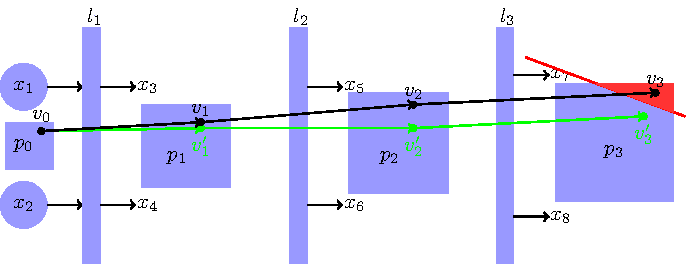
\includegraphics[scale=0.75]{fig/pictorial1.pdf}
    \caption{Pictorial representation of our approach on example in figure~\ref{fig:motivating}}
    \label{fig:pictorial1}
\end{figure}


% \begin{figure}[!ht]
% 	\centering
% 	\scalebox{0.55}{\documentclass[]{standalone}
\usepackage{tikz}
\begin{document}
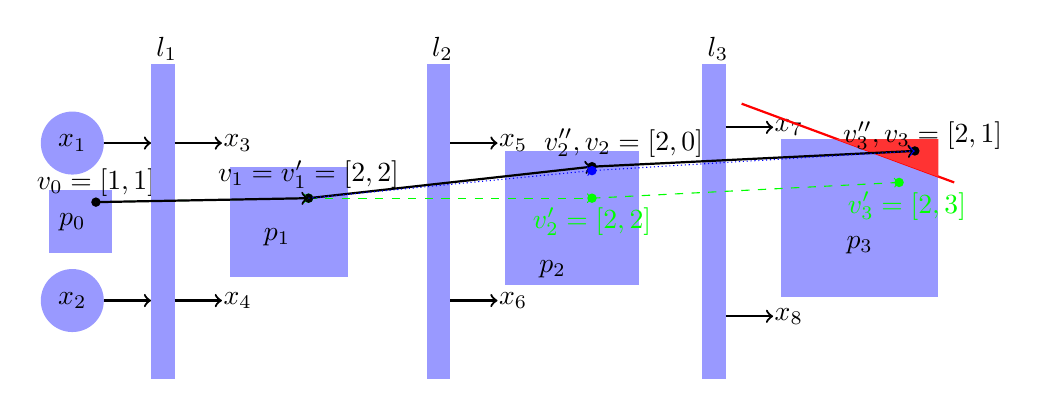
\begin{tikzpicture}
    \fill[blue!40!white] (3,3) circle (4mm);
    \fill[blue!40!white] (3,3) circle (0mm) node[color=black] {$x_1$};
    \fill[blue!40!white] (3,1) circle (4mm);
    \fill[blue!40!white] (3,1) circle (0mm) node[color=black] {$x_2$};
    \fill[blue!40!white] (2.7,1.6) rectangle (3.5,2.4);
    \fill[blue!40!white] (3,2) circle (0mm) node[color=black] {$p_0$};
    \fill[black] (3.3,2.25) circle (.6mm);
    \fill[blue!40!white] (3.3,2.5) circle (0mm) node[color=black] {$v_0 = [1,1]$};
    
    \draw[thick,->] (3.4,3) -- (4,3);
    \draw[thick,->] (3.4,1) -- (4,1);
    \fill[blue!40!white] (4,0) rectangle (4.3,4);
    \fill[blue!40!white] (5,1.3) rectangle (6.5,2.7);
    \fill[blue!40!white] (5.6,1.8) circle (0mm) node[color=black] {$p_1$};
    \draw[thick,->] (4.3,3) -- (4.9,3);
    \draw[thick,->] (4.3,1) -- (4.9,1);
    \fill[blue!40!white] (5.1,3) circle (0mm) node[color=black] {$x_3$};
    \fill[blue!40!white] (5.1,1) circle (0mm) node[color=black] {$x_4$};
    \fill[green] (6,2.3) circle (.6mm);
    \fill[black] (6,2.3) circle (.6mm);
    \fill[blue!40!white] (6,2.6) circle (0mm) node[color=black] {$v_1=v'_1=[2,2]$};
    % \fill[blue!40!white] (6,2) circle (0mm) node[color=green] {$v'_1$};
    \fill[blue!40!white] (4.2,4.2) circle (0mm) node[color=black] {$l_1$};

    \fill[blue!40!white] (7.5,0) rectangle (7.8,4);
    \fill[blue!40!white] (8.5,1.2) rectangle (10.2,2.9);
    \fill[blue!40!white] (9.1,1.4) circle (0mm) node[color=black] {$p_2$};
    \draw[thick,->] (7.8,3) -- (8.4,3);
    \draw[thick,->] (7.8,1) -- (8.4,1);
    \fill[blue!40!white] (8.6,3) circle (0mm) node[color=black] {$x_5$};
    \fill[blue!40!white] (8.6,1) circle (0mm) node[color=black] {$x_6$};
    \fill[green] (9.6,2.3) circle (.6mm);
    \fill[black] (9.6,2.7) circle (.6mm);
    \fill[blue!40!white] (10,3) circle (0mm) node[color=black] {$v''_2,v_2=[2,0]$};
    \fill[blue!40!white] (9.6,2) circle (0mm) node[color=green] {$v'_2 = [2,2]$};
    \fill[blue!40!white] (7.7,4.2) circle (0mm) node[color=black] {$l_2$};


    \fill[blue!40!white] (11,0) rectangle (11.3,4);
    \fill[blue!40!white] (12,1.05) rectangle (14,3.05);
    \fill[blue!40!white] (13,1.7) circle (0mm) node[color=black] {$p_3$};
    \draw[thick,->] (11.3,3.2) -- (11.9,3.2);
    \draw[thick,->] (11.3,.8) -- (11.9,.8);
    \fill[blue!40!white] (12.1,3.2) circle (0mm) node[color=black] {$x_7$};
    \fill[blue!40!white] (12.1,.8) circle (0mm) node[color=black] {$x_8$};
    \draw[red, thick] (14.2,2.5) -- (11.5,3.5);
    \fill[red!80!white] (12.7,3.05) -- (14,2.57) -- (14,3.05) -- cycle;
    \fill[black] (13.7,2.9) circle (.6mm);
    \fill[green] (13.5,2.5) circle (.6mm);
    \fill[blue!40!white] (13.8,3.1) circle (0mm) node[color=black] {$v''_3,v_3=[2,1]$};
    \fill[blue!40!white] (13.6,2.2) circle (0mm) node[color=green] {$v'_3 = [2,3]$};
    \fill[blue!40!white] (11.2,4.2) circle (0mm) node[color=black] {$l_3$};

    \draw[dashed,->,green] (3.3,2.25)  -- (6, 2.3);
    \draw[dashed,->,green] (6,2.3)  -- (9.6, 2.3);
    \draw[dashed,->,green] (9.6, 2.3) -- (13.5, 2.5);

    \draw[thick,->,black] (3.3,2.25)  -- (6, 2.3);
    \draw[thick,->,black] (6,2.3)  -- (9.6, 2.7);
    \draw[thick,->,black] (9.6, 2.7) -- (13.7, 2.9);



    %Following lines are for blue line
    % \draw[thick,->,blue] (3.3,2.25)  -- (6, 2.3);
    \fill[blue] (9.6,2.65) circle (.6mm);
    \draw[densely dotted,->,blue] (6,2.3)  -- (9.6, 2.65);
    \draw[densely dotted,->,blue] (9.6, 2.65) -- (13.7, 2.9);
    % \fill[blue!40!white] (9.9,2.6) circle (0mm) node[color=blue] {$v''_2 = [2,0]$};

\end{tikzpicture}

\end{document}
}
% 	\caption{Pictorial representation of our approach}
% 	\label{fig:pictorial}
% \end{figure}





%% \begin{figure}
%%     \begin{minipage}{0.9\textwidth}
%%         \centering
%%         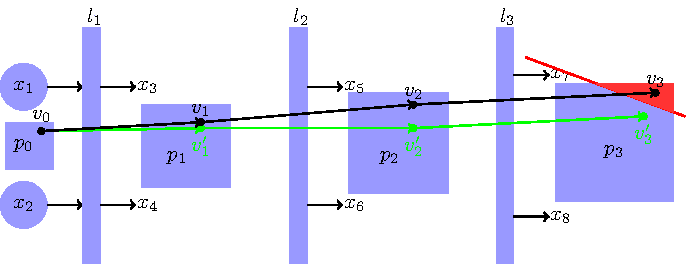
\includegraphics[scale=0.8]{fig/pictorial1.pdf}
        
%%         (a)
%%     \end{minipage}

%%     \begin{minipage}{0.9\textwidth}
%%         \centering
%%         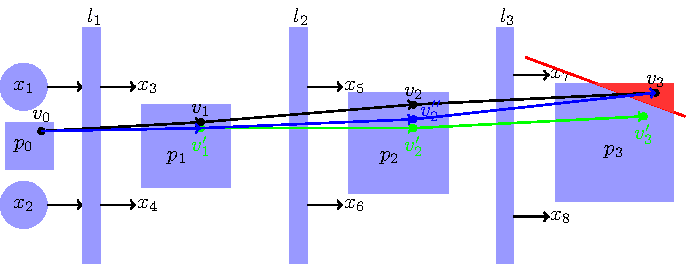
\includegraphics[scale=0.8]{fig/pictorial2.pdf}

%%         (b)
%%     \end{minipage}
%%     \caption{Pictorial representation of our approach}
%%     \label{fig:pictorial}
%% \end{figure}


%% Consider the pictorial representation of our approach in figure~\ref{fig:pictorial}. This pictorial representation is not 
%% related to the motivating example of figure~\ref{fig:motivating}. The shapes $p_0, p_1, p_2$, and $p_4$ represent 
%% the abstract constraints on each layer. We took the rectangle shape for simplicity,  but it is not necessarily a rectangle shape. 
%% The red zone on the output layer shows the intersection of the abstract constraints and the negation of the property. If this 
%% intersection is empty, we can say that the property was verified. Otherwise, we will get a path 
%% $v_0\rightarrow v_1\rightarrow v_2\rightarrow v_3$ as shown in figure~\ref{fig:pictorial}(a), which may or may not be a counterexample. 
%% We execute $v_0$ on neural network
%% and get path $v_0\rightarrow v'_1\rightarrow v'_2\rightarrow v'_3$ as shown in figure~\ref{fig:pictorial}(a). 
%% If the point $v'_3$ reaches the red zone, 
%% we report $v_0$ as a counterexample. Otherwise, we refine the path $v_0\rightarrow v_1\rightarrow v_2\rightarrow v_3$. 
%% To refine, we make the black line close to the green line from the first layer to the last layer so that the endpoints($v_0, v_3$)
%% remain unchanged. Here the closeness means making the neuron's values equal. 
%% First, we make the points $v_1$ close to $v'_1$, and it become completely equal (all neuron's values of $v_1$ become equal to the 
%% corresponding neuron's values of $v'_1$), we move on the the layer $l_2$. 
%% On layer $l_2$,
%% we make the points $v_2$ close to $v'_2$, and some neurons of $v_2$ become equal to the corresponding neurons of $v'_2$, and some
%% neurons could not become equal, so we got a new point $v''_2$ close to $v'_2$.  
%% Finally we got the path $v_0\rightarrow v'_1\rightarrow v''_2\rightarrow v_3$ in figure~\ref{fig:pictorial}(b) 
%% close to the green line.
%% We pick the layer where the blue line diverges first from the green line. Furthermore, get the neurons whose values are different 
%% from the green point's neuron's values. In figure ~\ref{fig:pictorial}(b), the first layer where blue line diverges from the 
%% green line is $l_2$.
%% We find all the neurons of points $v''_2$ and $v'_2$ whose values differ and mark them.     


% \begin{equation}
%     \begin{align}
%         \text{softConstrs} = \{x_5=2, x_6=0\}
%     \end{align}
% \end{equation}


%%% Local Variables:
%%% mode: latex
%%% TeX-master: "../main"
%%% End:
